%% main.tex — MSE Project Report: HiUni
%% Dokumentklasse msereport (1:1-Nachbau der Word-Vorlage template.docx).
%% Uebersetzen mit:  latexmk -pdf main.tex     (oder -lualatex fuer echtes Arial)
\documentclass{msereport}

% --- Architekturdiagramm (Abschnitt 3) --------------------------------------
\usepackage{tikz}
\usetikzlibrary{arrows.meta,calc,positioning}

% Umbruchstelle in langen Bezeichnern (ohne Trennstrich)
\newcommand{\bk}{\allowbreak}

% Rahmen-/Fuellfarben der Diagrammschichten
\definecolor{diaui}{HTML}{4F46E5}     % UI
\definecolor{diavm}{HTML}{7C3AED}     % Presentation
\definecolor{diarepo}{HTML}{0F766E}   % Domain/Daten
\definecolor{diadata}{HTML}{B45309}   % Persistenz & Netzwerk
\definecolor{diaext}{HTML}{6B7280}    % externe Systeme
\definecolor{diafcm}{HTML}{B31B1B}    % eigener Push-Server

\tikzset{
  dbox/.style={draw=#1, line width=0.3pt, fill=#1!10, rounded corners=2pt,
               anchor=north west, align=left, inner xsep=3pt, inner ysep=3pt,
               text=msetext, font=\fontsize{6.4pt}{7.4pt}\selectfont},
  dui/.style={dbox=diaui},
  dvm/.style={dbox=diavm},
  drepo/.style={dbox=diarepo},
  ddata/.style={dbox=diadata},
  dext/.style={dbox=diaext, font=\fontsize{6pt}{6.9pt}\selectfont},
  dfcm/.style={dbox=diafcm, dashed, font=\fontsize{6.2pt}{7.2pt}\selectfont},
  arr/.style={draw=msetext, line width=0.3pt,
              -{Stealth[length=3.4pt,width=2.4pt]}},
  lbl/.style={font=\fontsize{5.7pt}{6.6pt}\selectfont, text=msetext,
              fill=white, inner sep=1pt, align=left},
  lblr/.style={lbl, align=right},
  lay/.style={rotate=90, anchor=center, text=#1,
              font=\bfseries\fontsize{6pt}{6.9pt}\selectfont},
}

% Umbruch an bestehenden Bindestrichen erlauben (wie in Word); die
% Silbentrennung selbst bleibt aus, damit keine falschen deutschen
% Trennstellen entstehen.
\AtBeginDocument{\exhyphenpenalty=50\relax}

\hypersetup{
  pdftitle={HiUni: MSE Project Report},
  pdfauthor={Kjell Karstens, Johann Brosthaus},
}

\begin{document}

% ===========================================================================
%  Titelblock
% ===========================================================================
\msetitleblock{Project Report}{HiUni: Campus App for the University of Hildesheim}

{\mseleadfont Team:}
\par\vspace{10pt}

\begin{msetblr}[l]{
  colspec={Q[l,wd=5.6304cm] Q[l,wd=10.0330cm]},
  row{1}={bg=msetablered},
}
  Name & Student ID \\
  Kjell Karstens & 403556 \\
  Johann Brosthaus & 397592 \\
\end{msetblr}

% ===========================================================================
\section{Use Case}
% ===========================================================================

\begin{itemize}
  \item \textbf{Problem statement:} Students at the University of Hildesheim
        use a dozen digital services every day: canteen menu,
        LSF grade overview, Learnweb submissions, library room booking,
        university sports, campus cinema, university mail, timetable. They all
        live on separate websites, without a central overview and without a
        universal login. Anyone who checks food, submissions or mail several
        times a day signs in to each service anew, and does so on a smartphone
        that most of these sites were never made for.
  \item \textbf{Motivation:} We wanted the services we ourselves need several
        times a day in one place, and in a form that other students can use too.
        Comparable apps exist (e.\,g.\ Studo), but they do not cover the
        University of Hildesheim in the depth that really simplifies everyday
        life: no LSF grades, no group-room booking, no university mailbox. And
        the project was the chance to try out the MSE content (Android
        architecture, Compose, Lifecycle, persistence, testing) on a problem
        that affects us directly.
  \item \textbf{Real-world relevance:} The target picture from our project
        description reads: ``A student at the University of Hildesheim should
        know within ten seconds of launching the app what she has to do today,
        what is on offer in the canteen, which mails are unread and which
        submissions are due, without having to sign in anywhere again.'' Today
        this takes five websites and four logins.
  \item \textbf{Deliberate scope limits:} HiUni is \emph{not} a replacement for
        LSF and Learnweb: the app aggregates public content and login sessions;
        where a real administrative action is required (sports-course
        registration), it points to the official page. It is also not a rating
        platform and not an application run by the university IT department, but
        a private student project within the MSE module, not coordinated with
        the university IT. Cross-platform was deliberately not chosen: native
        Android was the course requirement and the learning goal.
\end{itemize}

\msegap

% ===========================================================================
\section{UX Design and Target Group}
% ===========================================================================

\subsection{Target Group}

\begin{itemize}
  \item \textbf{Primary users:} Students at the University of Hildesheim, across
        all semesters and degree programs. Deliberately scoped broadly, because
        canteen, mail, timetable and library are independent of the degree
        program.
  \item \textbf{Secondary users:} Staff with a teaching assignment who eat in
        the canteen or check their university mailbox; usable, but not the
        design focus, since exam, grade and submission features are tailored to
        students.
  \item \textbf{Explicitly not the target group:} Students at other
        universities (all endpoints, scrapers and credentials are specific to
        the University of Hildesheim) and iOS users.
  \item \textbf{User needs (today's workaround in parentheses):} Know what is on
        today (LSF timetable in the browser, no daily overview); see the canteen
        menu (separate STW-ON website); check unread mail (dedicated webmail
        login with the RZ account); keep an eye on submissions (Learnweb, CAS
        login on every visit); get an overview of grades and average (LSF grade
        report, aggregate in your head); find and book a free group room (ubwww
        with its own session handling); find a sports course (HSP program page,
        booking behind its own login).
  \item \textbf{Usage scenario (our own phrasing of the target picture from
        Section 1):} A student opens HiUni on the bus in the morning. On the
        home screen she sees the next lecture with a countdown and room, below
        it today's canteen offer, the unread mails and the next submission due.
        She taps the submission, sees the deadline, and books herself a group
        room for the afternoon on the way, without signing in to four portals.
\end{itemize}

\subsection{Mockups}

\begin{itemize}
  \item The design reference was a high-fidelity HTML/CSS mock
        (\emph{Uni Hi.html}) with 17 screens, produced with \emph{Claude Design}
        and sharpened by hand; the AI reflection on it is in Section 4.2. From
        it we translated the color system (OKLCH values as sRGB constants), the
        typography scale, the corner radii and the home layout into the Compose
        theme.
  \item The three core workflows in the following table come from it; the images
        are rendered directly from the mock.
\end{itemize}

\msegap

\begin{msetblr}[l]{
  colspec={Q[l,wd=3.4572cm] Q[l,wd=6.2794cm] Q[l,wd=5.5033cm]},
  row{1}={bg=msered2},
  cells={font=\msesmallfont},
}
  Screen & Mockup & Addresses which user need? \\
  Home (daily overview) & 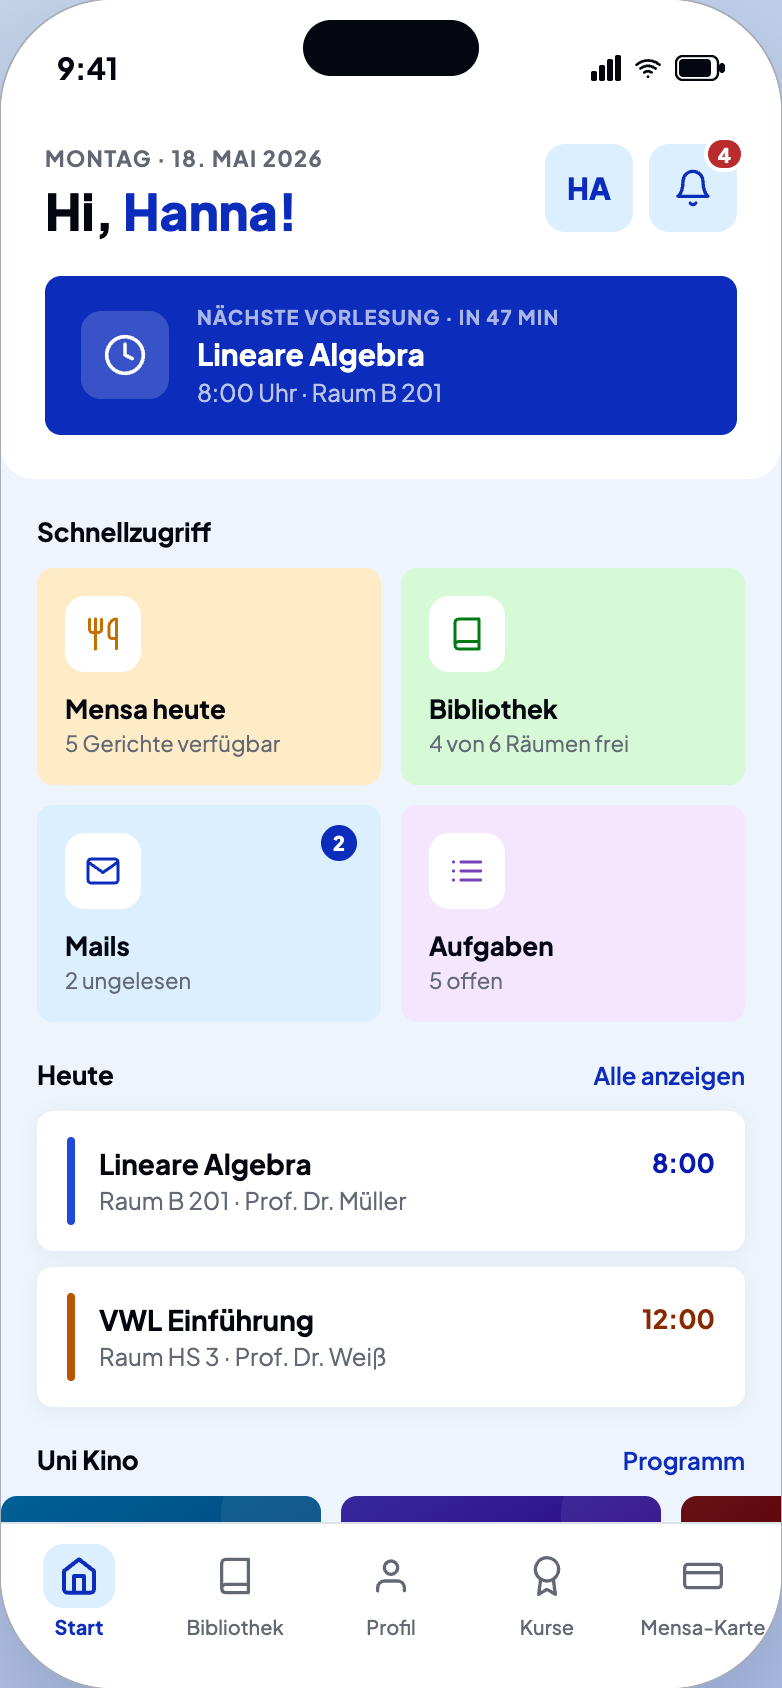
\includegraphics[width=2.35cm]{assets/mock-home.png} & Daily overview without multiple logins in one screen: what is on, what there is to eat, what is open \\
  Library / group room & 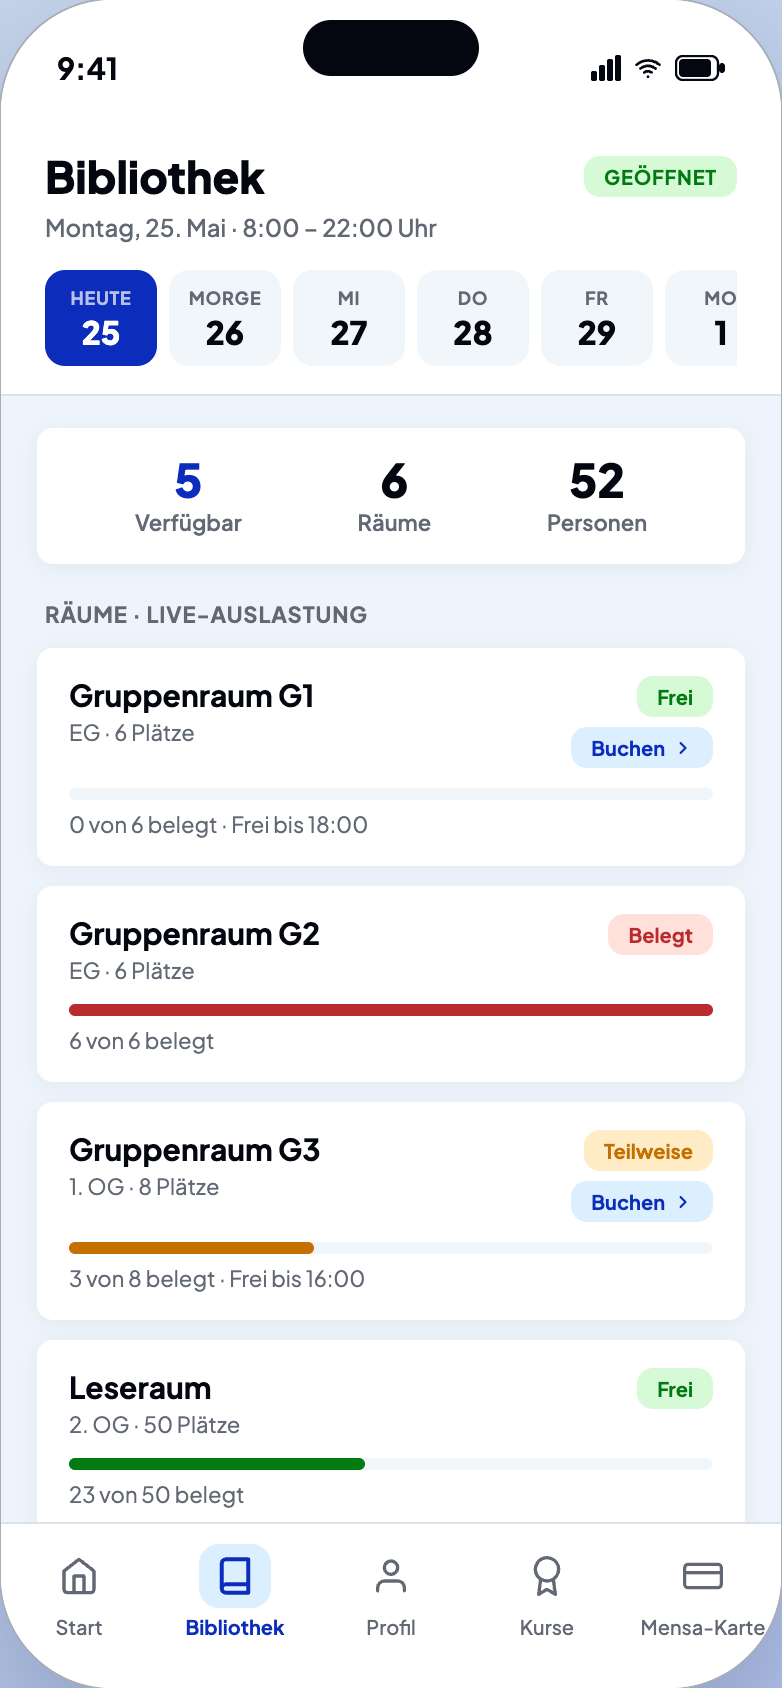
\includegraphics[width=2.35cm]{assets/mock-bib.png} & Find a free study room and book it directly, instead of operating the ubwww page on the phone \\
  Tasks and grades & 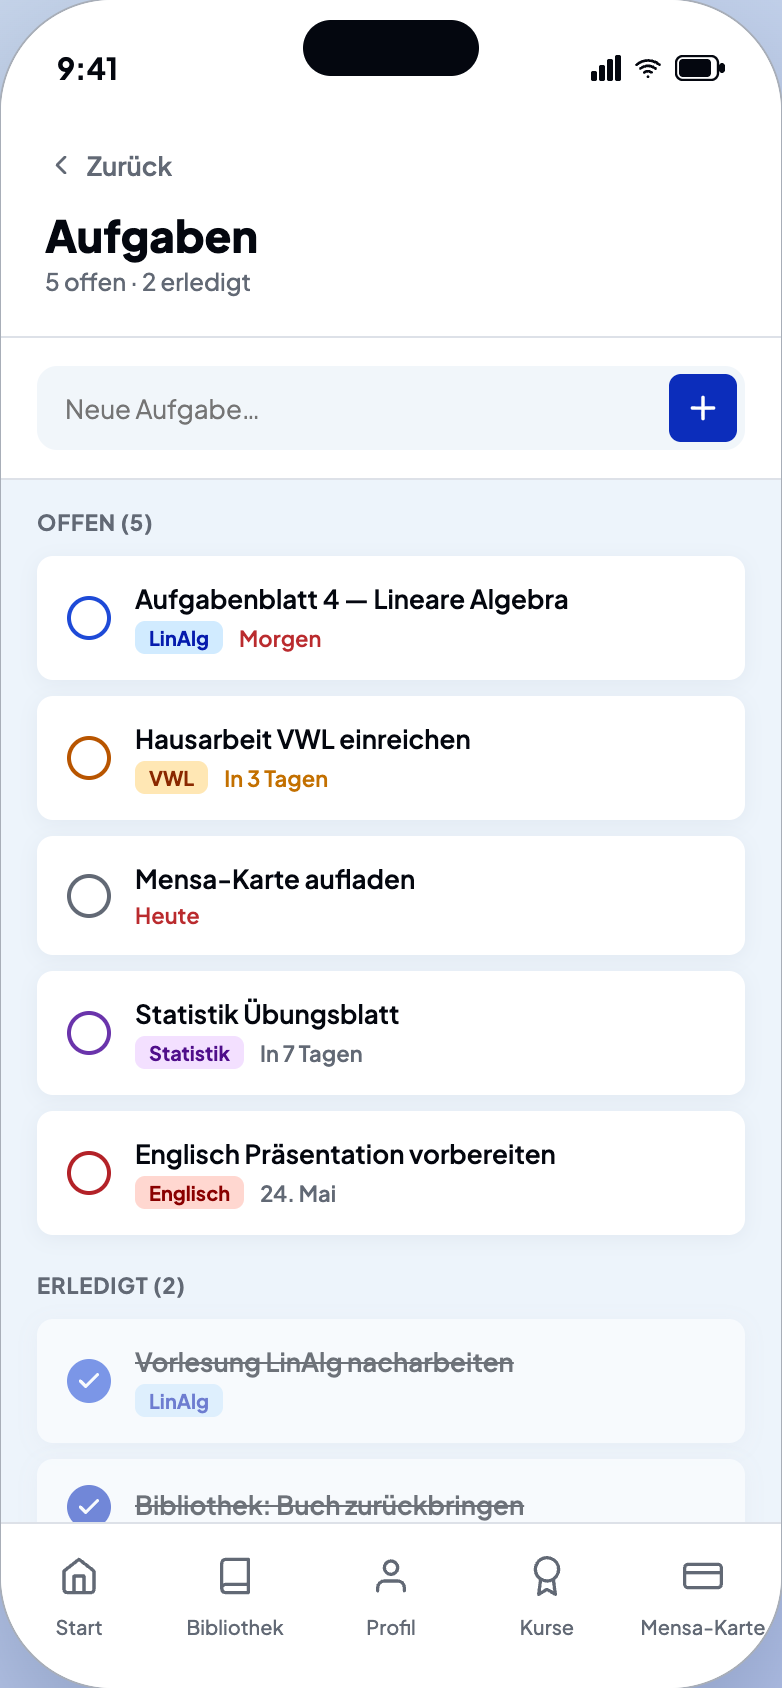
\includegraphics[width=2.35cm]{assets/mock-todo.png}\hspace{4pt}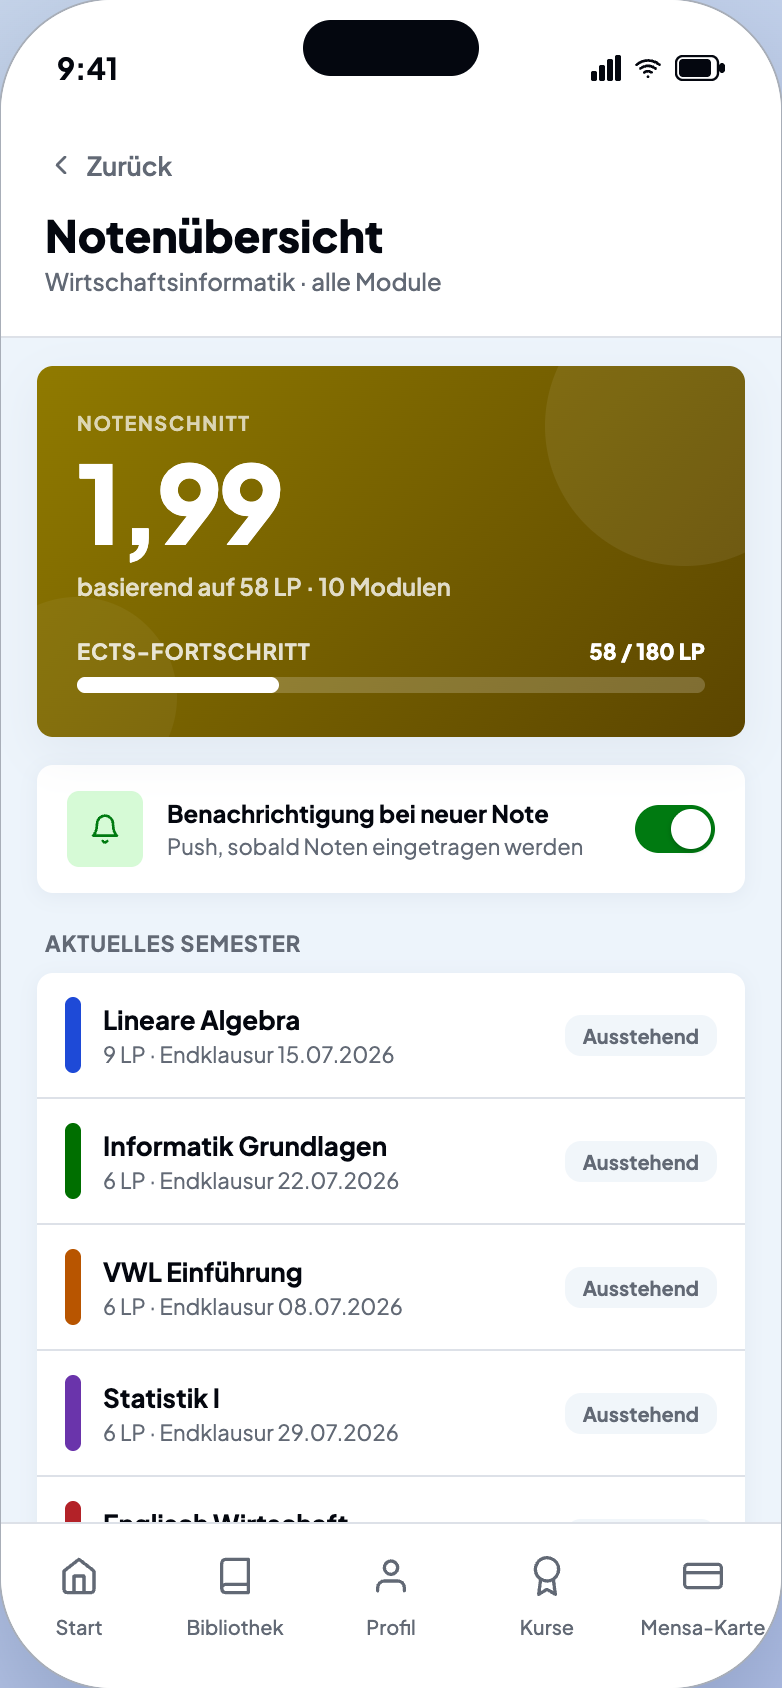
\includegraphics[width=2.35cm]{assets/mock-noten.png} & Submissions and grades at a glance, without logging in via CAS on every visit \\
\end{msetblr}

\msevspace{10pt}\mseblank

\subsection{Design Rationale}

\begin{itemize}
  \item \textbf{Deliberately omitted or simplified:} The mock had 17
        screens; we started with eight navigation destinations (Home, Calendar,
        Canteen, Cinema, Library, Mail, Settings, About). Exams, grades, sports
        and the push center followed later; study groups and a campus map are
        not built: the remaining effort did not fit the time budget, and study
        groups without a backend would have stayed a local note list. We dropped
        the in-app tweaks panel (accent color, greeting text) because it would
        have duplicated the settings. The About screen deliberately remained a
        minimal stub.
  \item \textbf{Design system instead of stock components:} We rebuilt pills,
        badges and the ``pillow'' indicator of the bottom navigation from
        \texttt{Surface} and \texttt{Text} by hand, rather than taking
        Material 3 components with a different look. It costs more code, but it
        keeps spacing, radii and color roles consistent across all screens.
  \item \textbf{A UX decision against the AI proposal:} For the day view of the
        calendar the AI generated a full hourly grid from 8:00 to 22:00 with
        per-event position calculation. In the pair review we rejected this as
        over-engineered for that project phase and reduced it to an agenda list;
        the rest of the feature wave mattered more than a pretty day view. In a
        later polish phase a color-coded hourly grid (8:00--18:00) did arrive
        after all. So the proposal only came too early, and in review we have
        since also checked whether something fits the current project phase.
\end{itemize}

\msegap

% ===========================================================================
\section{System Architecture Diagram}
% ===========================================================================

% Diagramm gemeinsam mit KI entworfen, von Hand nachgeführt — Anpassungen:
% Boxen/Pfeile hier direkt editierbar.
% Geometrie: alle Knoten mit anchor=north west an festen (x,y)-Positionen in cm,
% Schichten bei y = 0 / -2.70 / -5.30 / -7.85 / -11.70.
{\hbadness=10000 \hfuzz=30pt
\begin{tikzpicture}[x=1cm, y=1cm]

  \tikzset{
    bignode/.style={font=\fontsize{7.4pt}{8.8pt}\selectfont},
    biarr/.style={arr, {Stealth[length=3.4pt,width=2.4pt]}-{Stealth[length=3.4pt,width=2.4pt]}},
  }

  % ---------- Schicht-Beschriftungen (links) --------------------------------
  \node[lay=diaui]   at (0.30,-0.55) {UI};
  \node[lay=diavm]   at (0.30,-2.55) {Presentation};
  \node[lay=diarepo] at (0.30,-4.55) {Domain};
  \node[lay=diadata] at (0.30,-6.75) {Data \& Infra};
  \node[lay=diaext]  at (0.30,-9.65) {External};

  % ---------- Schicht 1: UI -------------------------------------------------
  \node[dui, bignode, text width=13.6cm, minimum height=1.05cm] (UI) at (0.9,0)
    {{\bfseries Compose UI (Single Activity) + Glance home widgets}\\
     render \texttt{UiState}, send user actions; widgets read repository flows directly};

  % ---------- Schicht 2: ViewModels ----------------------------------------
  \node[dvm, bignode, text width=13.6cm, minimum height=1.05cm] (VM) at (0.9,-2.0)
    {{\bfseries Feature ViewModels (\texttt{@HiltViewModel}), incl.\ HomeViewModel}\\
     hold one \texttt{UiState} per screen as a StateFlow, call repository functions};

  % ---------- Schicht 3: Repositories --------------------------------------
  \node[drepo, bignode, text width=13.6cm, minimum height=1.05cm] (REPO) at (0.9,-4.0)
    {{\bfseries Feature repositories as the single source of truth}\\
     TTL refresh, mapping HTML/JSON to Room entities, expose flows upward};

  % ---------- Schicht 4: Daten \& Infrastruktur -----------------------------
  \node[ddata, bignode, text width=6.5cm, minimum height=1.35cm] (STORE) at (0.9,-6.0)
    {{\bfseries Room + SQLCipher, DataStore}\\
     encrypted DB (schema 35, 34 migrations),\\
     settings and credentials};

  \node[ddata, bignode, text width=6.5cm, minimum height=1.35cm] (NET) at (8.0,-6.0)
    {{\bfseries Network, WorkManager, CasSession}\\
     OkHttp + Jsoup scraper, background workers,\\
     CAS SSO with silent renewal};

  % ---------- Schicht 5: externe Systeme -----------------------------------
  \node[dext, bignode, text width=9.6cm, minimum height=1.15cm] (EXT) at (0.9,-9.0)
    {{\bfseries University systems (no API, via scraping / protocol)}\\
     LSF + CAS, Learnweb, STW canteen, ubwww library, university mail (IMAP/SMTP)};

  \node[dfcm, bignode, text width=3.5cm, minimum height=1.15cm] (FCM) at (11.0,-9.0)
    {{\bfseries FCM tickle server}\\
     (FastAPI; deployment\\ pending)};

  % ---------- Pfeile --------------------------------------------------------
  \draw[biarr] (7.0,-1.05) -- (7.0,-2.0);
  \node[lbl, anchor=west] at (7.15,-1.52) {$\downarrow$ actions \quad $\uparrow$ UiState (StateFlow)};

  \draw[biarr] (7.0,-3.05) -- (7.0,-4.0);
  \node[lbl, anchor=west] at (7.15,-3.52) {$\downarrow$ \texttt{refresh()} \quad $\uparrow$ \texttt{Flow<Entity>}};

  \draw[biarr] (3.5,-5.05) -- (3.5,-6.0);
  \node[lbl, anchor=west] at (3.65,-5.52) {Query / \texttt{upsert}};

  \draw[arr] (11.2,-5.05) -- (11.2,-6.0);
  \node[lbl, anchor=west] at (11.35,-5.52) {trigger sync};

  \draw[arr] (9.3,-7.35) -- (9.3,-9.0);
  \node[lblr, anchor=east] at (9.15,-8.1) {HTTPS, CAS cookie,\\scraping (rate-limited)};

  \draw[arr, dashed] (12.7,-9.0) -- (12.7,-7.35);
  \node[lbl, anchor=west] at (12.85,-8.1) {silent tickle\\(planned)};

\end{tikzpicture}
\par}
\vspace{4pt}
{\msesmallfont\itshape How to read it: arrows pointing down are calls, arrows
pointing up are data streams (flows).\par}

\subsection{Architecture Justification}

\begin{itemize}
  \item \textbf{Why this structure?} The app is strictly layered (Compose
        $\to$ ViewModel $\to$ Repository $\to$ Room/network), but packaged
        \emph{feature-first}: each of the 21 feature packages bundles
        entities, DAOs, repositories, ViewModels and screens in one place. The
        repository is the single source of truth; the UI never reads from the
        network, only from Room flows, which is why every screen has content
        instantly and the app stays usable offline. Cross-feature access is
        forbidden by convention, with two documented exceptions:
        \texttt{feature.home} (combines eleven repositories) and
        \texttt{feature.widgets} (Glance has no ViewModels). Because five
        external systems are integrated via HTML scraping (LSF, Learnweb, ubwww,
        unifilm, university sports), the HTTP client, the politeness throttle,
        the CAS session and the background workers sit outside the features;
        otherwise every scraper would carry its own rate-limit and session
        logic. The FCM tickle server is deliberately a separate, content-free
        box: it knows only device tokens and sends a pure ``go check''
        impulse, so that no credentials or mail content ever touch a foreign
        server. It is implemented and tested but not yet deployed to production;
        until then the mail sync runs via the periodic WorkManager workers.
        Security-critical data lives in a SQLCipher-encrypted Room database with
        a key from the Android Keystore.
  \item \textbf{Rejected alternatives:} (1) \emph{Layer-first with several
        Gradle modules}: a single module builds faster at our size and the
        feature ownership does not fray; the price is missing compile-time
        isolation, but the packages map one to one. (2) \emph{Retrofit + Moshi}:
        not worth it for a handful of JSON endpoints alongside mostly HTML
        scraping; OkHttp plus kotlinx.serialization suffice. (3) \emph{Koin
        instead of Hilt}: saves boilerplate, but costs the compile-time check of
        the dependency graph. (4) \emph{One shared calendar table}: the
        discriminator approach breaks the feature separation, so pinned entries
        are now snapshots in their own table. (5) \emph{AGP 9}: Hilt broke
        completely with it, back to AGP 8.7 + Kotlin 2.0 + KSP1.
  \item \textbf{Walk-through (scenario from 2.1: ``open the app in the
        morning''):} (1) The tickle server is meant to send a silent,
        high-priority FCM data message with no payload every 15 minutes (server
        built, deployment pending; currently the periodic worker starts
        instead). (2) The \texttt{HiUniMessagingService} receives it, obtains
        its dependencies via a Hilt \texttt{EntryPoint} (Firebase instantiates
        it itself), checks preconditions and enqueues an \emph{expedited}
        \texttt{MailPushSyncWorker}; the service does not do the work, because
        its process can end immediately. (3) The worker calls
        \texttt{EmailRepository.refresh()} and classifies network errors as
        \texttt{retry} and auth errors as \texttt{failure}; in parallel the
        \texttt{LsfSyncWorker} obtains a service ticket via \texttt{CasSession}
        with silent renewal. (4) All HTTP calls go through the shared OkHttp
        client with a cookie jar and a \texttt{PolitenessInterceptor}; Jsoup
        parses HTML, kotlinx.serialization the canteen response. (5) Results are
        upserted into Room, a single write that all observers hang off; the DAOs
        emit new flows, the repositories pass them on. (6) The
        \texttt{HomeViewModel} combines the flows from eleven feature
        repositories (calendar, canteen, mail, tasks, \dots) into a
        \texttt{HomeUiState}. (7) The \texttt{HomeScreen} collects it
        \texttt{withLifecycle} and draws the banner, canteen card and mail
        badge; the timetable widget reads the same flow via the widget
        EntryPoint.
\end{itemize}

\subsection{Third-Party Libraries}

In one sentence: Hilt wires the app together, Room and SQLCipher store it
encrypted, OkHttp and Jsoup fetch and parse the university pages, Jakarta Mail
speaks IMAP/SMTP, kotlinx.serialization and biweekly read JSON and iCal, Coil
loads images, Firebase provides the push transport, and MockK/Turbine/Robolectric
carry the tests. Everything below solves exactly one task that you would
otherwise have to build yourself.
\par\vspace{6pt}

{\itshape Alongside the platform building blocks from Google/AndroidX (Compose,
Navigation, Lifecycle, DataStore, WorkManager, Glance, Biometric, Window/WindowSizeClass,
Fragment for BiometricPrompt, SplashScreen, Palette for poster colors, Material Icons,
Google Fonts) and the Kotlin coroutines, which we count as part of the architecture
decision rather than as third-party libraries, the following third-party libraries are
in use. In addition, but without effect on the domain logic: Timber (logging) and LeakCanary
(debug build only).\par}
\vspace{6pt}

\begin{msetblr}[l]{
  colspec={Q[l,wd=3.8100cm] Q[l,wd=5.7150cm] Q[l,wd=5.7150cm]},
  row{1}={bg=msered2},
  cells={font=\msesmallfont},
}
  Library & Purpose & Why this one (over alternatives)? \\
  Hilt / Dagger 2.56 & DI, \texttt{@HiltViewModel}, \texttt{@HiltWorker}, EntryPoints for widgets and the push service & Compile-time check of the dependency graph instead of runtime surprises \\
  Room 2.6.1 (+ KSP) & SQLite access, one AppDatabase, entities and DAOs in the feature, versioned migrations & Type-safe queries and Flow integration; KSP1, because Room 2.6.1 does not compile with KSP2 \\
  SQLCipher (sqlcipher-android 4.6.1) & Encryption of the entire Room database & Mail cache, grades and exam data sit on disk; prefs alone leave the DB open \\
  OkHttp 4.12 (+ logging interceptor) & HTTP client for scrapers and APIs, cookie jar, cache, politeness interceptor & Cookies, pool and cache built in; with \texttt{HttpURLConnection} that would be manual work \\
  Jsoup 1.18.1 & HTML parsing for LSF, Learnweb, ubwww, unifilm, university sports & Robust CSS selectors on broken university HTML instead of regex \\
  Angus Mail 2.0.3 / Jakarta Mail API 2.1.3 & IMAP and SMTP client of the mail feature & Protocol-correct including IDLE and SPECIAL-USE; a custom parser would be weeks of work \\
  kotlinx.serialization 1.7.3 & Type-safe DTOs for JSON endpoints (canteen, TMDB) & Kotlin-native, no reflection overhead; Retrofit/Moshi only pay off with more endpoints \\
  Coil 2.7.0 (coil-compose) & Asynchronous loading of the cinema posters & Cache, concurrency and Compose integration ready-made \\
  Firebase Cloud Messaging (firebase-bom 33.7.0) & Reception of the silent tickle data messages from our push server & The only way out of Doze without polling; only the transport is used, no analytics \\
  biweekly 0.6.8 & iCalendar parsing (RFC 5545) of the Learnweb feed as a second source for deadlines & Correct RRULE and EXDATE expansion is a project of its own \\
  MockK 1.13.13, Turbine 1.1.0, Robolectric 4.13 & Unit tests: Kotlin mocking, flow assertions, Android tests on the JVM & MockK understands Kotlin idioms, Turbine makes StateFlow tests readable, Robolectric saves the emulator \\
\end{msetblr}

\msegap

\subsection{The Tickle Server: Concept and Status}

Noticing new university mail quickly collides with Android: from Doze mode an
app may not check by itself every minute. The usual way out would be a server
that watches the mailboxes and, on new mail, sends a push message with content,
but then credentials and mail content would sit on foreign infrastructure. Our
\emph{tickle} server avoids exactly that: it knows only FCM device tokens, that
is, only ``which device can I push to'', and sends a silent, content-free,
high-priority data message every 15 minutes (\texttt{\{type: sync\_tickle\}}).
That wakes the device from Doze; the app realizes ``time to check'' and fetches
the mails itself via IMAP, with credentials that live only on the device. The
model is deliberately built like WhatsApp's: the push infrastructure knows only
that something is probably pending, not what. If the server fails or is
compromised, at most device tokens are affected, no mailboxes. On the server
side there are token purge (invalid tokens are dropped automatically), a rate
limit and an \texttt{X-Api-Key}. The server (FastAPI, around 300 lines,
Docker-ready) is implemented and tested but not yet deployed to production;
until then the periodic WorkManager worker handles the mail refresh. The FCM
keys (the server's service account, the app's \texttt{google-services.json}) are
deliberately not in the repo but excluded via \texttt{.gitignore} and injected
through environment variables or CI secrets; the repo holds only an
\texttt{.env.example} as a template. So a checkout intentionally contains no push
credentials.

\msegap

% ===========================================================================
\section{Developer Diary}
% ===========================================================================

This section shows the course of development: first the milestones, then the
collaboration with the AI with its successes and failures.
\par\vspace{6pt}

\subsection{Development Milestones}

\begin{msetblr}[l]{
  colspec={Q[l,wd=0.6350cm] Q[l,wd=1.8697cm] Q[l,wd=4.3392cm] Q[l,wd=4.3392cm] Q[l,wd=3.2103cm]},
  row{1}={bg=msered2},
  row{2-11}={font=\msesmallfont},
}
  \# & Date & Activity & Result & Issues \\
  1 & 2026-05-23 & Foundation: Gradle, Compose, Hilt, Room, DataStore, WorkManager, AdaptiveScaffold, 7 ADRs, stubs & \texttt{assembleDebug} and \texttt{lintDebug} green on the same day & KSP2 broke the Room annotations, rollback to KSP1 \\
  2 & 2026-05-24 & Calendar CRUD (list, day, week, reminder); canteen via the STW-ON API & Both done, test pattern for repositories in place & AI DTO of the canteen API with invented field names; day view over-engineered \\
  3 & 2026-05-26 & Library group rooms: floor plan, slot picker (max.\ 2 h), session, book and cancel & Booking flow in the app instead of the browser & Session-fixation bug in the real ubwww; report to the library pending \\
  4 & 2026-05-31 & Scraper wave: cinema, library occupancy, mail (IMAP/SMTP); sports followed at the end of June & All three in; library/sports (Johann), mail/cinema (Kjell) & IMAP folder names differ per server; fix via SPECIAL-USE \\
  5 & 2026-06-27 & Tablet foundations (rail, drawer, multi-pane); on the side, as an experiment, P2P canteen ratings (Ed25519, Ktor relay) & Adaptive layouts everywhere; the ratings stayed an unmerged experiment and were dropped & BottomSheet on BottomSheet did not stack; percentage value truncated \\
  6 & 2026-06-29 & Learnweb in four stages: CAS SSO, course list, submission deadlines in the calendar, iCal & Complete in one day, reminders 3 d / 1 d / 2 h & Reminders first in the generic event category, own one from 17.07.\ \\
  7 & 2026-07-13 & Five Glance widgets plus a design kit and deep links, Ultracode in parallel in worktrees & All five shipped, around 600 lines of layout replaced by the kit & Glance limit of 10 children undetected for four days (silent exception) \\
  8 & 2026-07-16 & Grades and average from the LSF grade report, offline marking & Grades screen live, test suite 140 $\to$ 289 & Fixture with real exam data, now synthetic with a data-protection assertion \\
  9 & 2026-07-16 & FCM tickle server (FastAPI) for mail push without credentials or content & Implemented, Coolify deployment prepared (service account as an env variable); deployment pending & Rate limit and token age added only afterwards \\
  10 & 2026-07-17 & Grade report linked to courses (course number), semester anchor for the icon, Glance fix, Learnweb channel & Four commits in one day, 475 tests, 0 failures & Precedence of manual grade over grade report secured \\
\end{msetblr}

\msevspace{10pt}\mseblank

\subsection{AI Interaction Log: Critical Incidents}

The whole project was created with \emph{Claude Code} (Anthropic, model Opus 4.x
with a 1M-token context), but deliberately not in a question-and-answer style.
The division of roles has been in an \texttt{AI\_USAGE.md} in the repo since day
one: the AI wrote around 80\,\% of the raw code, we made the architecture,
library and scope decisions. The seven ADRs came about the same way: phrasing
drafts from the AI, decided in conversation. Two operating modes of Claude Code
were decisive here and go beyond mere dictation: the \emph{Superpowers} skills in
planning and the \emph{Ultracode} mode in implementation.

\textbf{Planning ran AI-assisted too.} The \emph{Superpowers} skills are
reusable work instructions that impose discipline on the agent before it writes
code. The ratings feature makes this traceable: from a \texttt{brainstorming}
dialogue a 654-line design spec emerged on 28.06., iterated over the afternoon in
five commits, with a section ``Resolved points (decided in brainstorming)'' and
the removal of an entire phase (LAN sync via mDNS) after research showed that
Eduroam blocks multicast. From it the \texttt{writing-plans} skill produced an
implementation plan of 3\,344 lines: 7 phases, 34 tasks, each a TDD three-step
(failing test, implementation, commit). What matters to us is the separation: the
spec is the document \emph{we} decided on, the plan only its mechanical
unfolding.

\textbf{Implementation ran twice in \emph{Ultracode} mode}, that is, as
multi-agent orchestration across separate Git worktrees. The first use
accompanied the later-dropped ratings experiment (28.06.): two agents built in
parallel, plan-driven, and after each phase a review ran across the whole branch.
Fully traceable in the history of \texttt{main} is the second use, the widgets
(13.07.): between the Glance foundation and the last merge lie, according to Git
timestamps, 63 minutes with 19 commits and around 2\,900 inserted lines. The
sequence is readable in the history: foundation sequential, three of the five
widgets in their own agent worktrees (the main session built two directly), then
a shared design kit and three further worktrees that switched the finished
widgets over to it; their merges have \emph{negative} net diffs, because the kit
replaces duplicated layout. A human merged throughout: all merge commits carry
the same author, a manifest conflict is documented there and was resolved by
hand. On top of that came an automated \texttt{/code-review} per branch before
the merge.

The following five incidents are the ones we learned the most from.

\msevspace{6pt}\mseblank

\begin{msetblr}[l]{
  colspec={Q[l,wd=0.4586cm] Q[l,wd=1.6933cm] Q[l,wd=4.3392cm] Q[l,wd=3.9511cm] Q[l,wd=3.9511cm]},
  row{1}={bg=msetablered},
  row{2-6}={font=\msesmallfont},
}
  \# & Milestone & What happened & AI's output (brief) & Your action / validation \\
  1 & 3 (Library) & Two \texttt{Set-Cookie} headers in the booking flow; session logic analyzed with the AI & ubwww rotates the PHPSESSID after the CAS login but does not invalidate the old session: ``one booking per day'' can be bypassed, leaving orphaned reservations & Reproduced with curl and DevTools in a bug document; the client now takes the \emph{last} cookie. Report to the library IT pending \\
  2 & 7 (Widgets) & In the exam-countdown widget the room was missing in the large size, without a crash & \texttt{MetaChip} placed icon, spacing and text as three siblings in the row: 11 children where Glance allows 10; every render threw a silent \texttt{IllegalArgument\bk Exception} & Chip wrapped into a row wrapper (one child), \texttt{WidgetLimits} with the limit and a unit test; the AI does not know such framework limits \\
  3 & 5 (Ratings) & Approval percentage of the aggregated canteen ratings & \texttt{(positive * 100) / total} as the ``correct'' formula, i.e.\ integer division that truncates instead of rounding & Only caught while writing the tests; fix and edge-case tests in the ratings experiment, test-first since then \\
  4 & 2 (Canteen) & DTO for the STW-ON canteen API, for which there is no public documentation & Invented field names (\texttt{prices}, \texttt{notes} instead of \texttt{price} and a nested \texttt{tags}): compiled cleanly, returned empty lists & Live call with curl, JSON sample into the repo, DTO corrected. Since then, inspect first, then generate \\
  5 & 7 (Widgets) & Five widgets in one day, Ultracode in parallel in separate Git worktrees & Each worktree delivered a working widget, but with its own style: colors, paddings, structures & Throughput impressive, then a unification pass to one widget theme. A design kit belongs \emph{before} the parallelism \\
\end{msetblr}

\msegap

\subsection{Project Documentation}

The development process is documented in the repo, not only in the code. The
most important artifacts:

\begin{itemize}
  \item \texttt{docs/adr/} \textbf{(ADR 0001--0007):} one architecture
        decision each on feature-first packages, single-activity Compose, Hilt,
        one AppDatabase, library strategy, ``no unified calendar'' and
        AGP 8.7; the AI supplied drafts, the team decided.
  \item \texttt{docs/process/} \textbf{(01--07):} project description,
        architecture overview, chronological engineering log, AI workflow
        (disclosure plus prompt log and reflection), build instructions,
        team/contributions, interim pitch.
  \item \texttt{docs/superpowers/} \textbf{spec and plan:} the 654-line design spec
        and the 3\,344-line implementation plan derived from it for the
        ratings feature (see Section 4.2).
  \item \texttt{.superpowers/sdd/} \textbf{execution logs:} the task-by-task
        record of the subagent-driven run (per-task brief and report, the
        \texttt{progress.md} with the Opus review verdicts, the whole-branch
        review reports), i.e.\ the traceable execution trail behind that plan.
  \item \textbf{Repo root:} \texttt{AI\_USAGE.md} (living AI disclosure, updated
        per commit wave), \texttt{CHANGELOG.md},
        \texttt{docs/FEATURES.md} (feature status), \texttt{docs/DEVELOPMENT.md}
        (internal cookbook) as well as the concept and plan files of the initial
        phase (\texttt{HIUNI\_KONZEPTE}, \texttt{-LIBRARIES}, \texttt{-REFACTOR-PLAN}).
\end{itemize}

\msegap

% ===========================================================================
\section{Android Features Report}
% ===========================================================================

\subsection{Features Used}

The app uses the following platform building blocks. ``Why'' names the concrete
requirement in each case, not just the technology.
\par\vspace{6pt}

\begin{msetblr}[l]{
  colspec={Q[l,wd=3.4572cm] Q[l,wd=5.8913cm] Q[l,wd=5.8913cm]},
  row{1}={bg=msetablered},
  cells={font=\msesmallfont},
}
  Feature & Where it's used (screen/class) & Why this feature was needed \\
  Activity lifecycle, intents and deep links & \texttt{MainActivity} (\texttt{FragmentActivity}, \texttt{singleTask}), \texttt{onCreate}/\texttt{onNewIntent}, \texttt{Widget-} and \texttt{NotificationDeepLinkController} & Single activity with one Compose NavGraph; widget, notification and NFC intents land in the running instance and are mapped to a navigation destination \\
  Local database: Room with SQLCipher & \texttt{AppDatabase} (schema 35), entities and DAOs per feature, \texttt{Migrations.kt} & Offline-first: every screen reads from the DB, never from the network. Encrypted, because the mail cache and grades sit in it \\
  Schema migrations & 34 additive \texttt{Migration} objects, schema export to \texttt{app/schemas} & No destructive migration: an app update must not delete user data \\
  DataStore (Preferences) & \texttt{SettingsDataStore} & Settings, sync intervals, navigation order and refresh timestamps, asynchronous without \texttt{SharedPreferences} blocking \\
  Encrypted preferences + Keystore & \texttt{CredentialsManager}, \texttt{DatabaseKeyProvider} (Encrypted\bk SharedPreferences) & Mail credentials and the 32-byte DB key must not sit in plaintext; master key in the Keystore \\
  Biometrics & \texttt{MailLockGate} (\texttt{BiometricPrompt}, \texttt{BiometricManager}) & The mail tab shows other people's communication, unlocked by fingerprint or device code; hence the \texttt{FragmentActivity} \\
  Runtime permissions & \texttt{OnboardingScreen}, \texttt{RemindersSettingsScreen} (\texttt{POST\_NOTIFICATIONS}), \texttt{canScheduleExactAlarms()}, NFC optional & Notifications from API 33, exact alarms opt-in from API 31; the app must run without either permission \\
  Notification channels and categories & \texttt{NotificationPresenter}, \texttt{NotificationCategory} plus an in-app push center & Events, grades, mail and system separately mutable; the in-app center logs independently of the OS permission \\
  AlarmManager & \texttt{NotificationScheduler} (\texttt{setExactAndAllowWhileIdle}) & Event, exam and submission reminders must fire on the right minute even in Doze \\
  WorkManager & \texttt{LsfSyncWorker}, \texttt{SportSyncWorker}, \texttt{MailPushSyncWorker}, \texttt{PushRegistrationWorker} (\texttt{@HiltWorker}) & Guaranteed background work despite Doze and battery optimization, with a network constraint and backoff \\
  Firebase Cloud Messaging & \texttt{HiUniMessagingService}, \texttt{MailTickleHandler} & Without push the app would have to poll every minute; the silent data message wakes it but carries no content \\
  App widgets with Glance & \texttt{feature.widgets} (five widgets), \texttt{WidgetHiltEntryPoint} & Timetable, canteen, tasks and exam countdown on the home screen without launching the app \\
  NFC (IsoDep) & \texttt{NfcScanController}, \texttt{MensaCardReader} & There is no API for the student card's balance, so ISO-14443-4 APDUs directly from the card \\
  WindowSizeClass / adaptive layouts & \texttt{AdaptiveScaffold}, \texttt{NavigationType} & The same program on phone and tablet: bottom bar, rail or drawer by width, including multi-pane \\
\end{msetblr}

\subsection{Implementation Details}

\begin{itemize}
  \item \textbf{NFC reader for the student card.} A singleton
        (\texttt{NfcScanController}) mediates between ViewModel and Activity
        via two \texttt{SharedFlow}s (detected tags, navigation request) and a
        \texttt{StateFlow} \texttt{scanning}. The \texttt{MainActivity}
        observes \texttt{scanning} in the \texttt{lifecycleScope} and turns on
        the foreground dispatch only then; \texttt{onPause} always disables it,
        \texttt{onResume} reactivates it only during a running scan, so the app
        does not ``steal'' a card that comes near the device outside the payment
        flow. Registration is explicit with \texttt{techLists = [IsoDep]},
        otherwise another tag technology blocks IsoDep (``only one TagTechnology
        can be connected at a time''). Two entry points: an external
        \texttt{ACTION\_TECH\_DISCOVERED} intent on a cold start (the controller
        sets \texttt{scanning} itself and navigates to the card screen) and the
        scan button in the screen. At the protocol level: DESfire over
        ISO-7816-4-wrapped APDUs, multiple frames via status \texttt{0xAF},
        UID from the anticollision rather than via a vendor command (current
        cards answer that with ``illegal command code'');
        \texttt{IsoDep.connect()} up to three times with 80/160 ms backoff.
  \item \textbf{Five Glance widgets.} Glance does not render into our process
        but into \texttt{RemoteViews}, so almost no app architecture applies
        here: a \texttt{GlanceAppWidget} cannot be an
        \texttt{@AndroidEntryPoint}, so the widgets obtain their four
        repositories via an \texttt{@EntryPoint} and
        \texttt{EntryPointAccessors.fromApplication}; without a ViewModelStore
        they collect the Room flows directly. Updates run not via the
        AppWidget timer (\texttt{updatePeriodMillis=0}) but via the
        flow emissions; interactive buttons run via \texttt{ActionCallback}
        with a subsequent \texttt{update()}. Colors must come as
        \texttt{ColorProvider(day, night)}, otherwise dark mode breaks,
        and a custom widget theme replaces \texttt{MaterialTheme}. The limit
        of 10 direct children per container has been a named constant with a
        test in the code since the silent rendering bug.
  \item \textbf{Push ``tickle'' plus background sync with CAS SSO.} The server
        sends no payload, only a type marker (server done, deployment
        pending; the app-side receive path is fully implemented). The
        decision logic (``should this tickle trigger a sync?{}'') is decoupled
        from Firebase and runs as a JVM test. The
        \texttt{FirebaseMessagingService} is instantiated by the SDK, not by
        Hilt, hence its own EntryPoint; it reads preconditions blocking, because
        the callback runs on a background thread anyway. Work happens in an
        \emph{expedited} \texttt{MailPushSyncWorker}
        (\texttt{RUN\_AS\_NON\_EXPEDITED} as a fallback, \texttt{KEEP} against
        tickle bursts), because the service process ends after the callback; the
        worker re-checks the credentials and classifies errors into
        \texttt{retry} and \texttt{failure}. The periodic
        \texttt{LsfSyncWorker} works through courses, timetable, exams and
        the grade report with a 400 ms throttle; auth errors are retried up to
        twice so the CAS session renews silently, a parse error does \emph{not}
        abort the run but produces a deduplicated warning in the push center
        (``exam dates outdated''). The most critical detail sits in the session:
        CAS binds the ticket-granting cookie to the user agent of the issuing
        WebView; without replaying it the server deletes it on the next request.
  \item \textbf{Edge cases.} \emph{Notification permission denied:} the entry
        always goes into the in-app push center, the system notification only
        with granted \texttt{POST\_NOTIFICATIONS}. \emph{No exact alarms:}
        fall back to \texttt{set()}. \emph{Offline:} the
        \texttt{ConnectivityObserver} requires \emph{internet} \emph{and}
        \emph{validated} (no captive-portal false alarm) and debounces 1{,}5 s,
        a banner above the NavHost shows the state centrally, a label marks
        stale data (offline or refresh older than 6 h). \emph{No NFC chip:} in
        the manifest \texttt{required=false}, the adapter may be \texttt{null}.
        \emph{Configuration change:} deep-link intents are voided after being
        consumed (\texttt{intent.action = null}), the scaffold reacts live to
        the new \texttt{WindowSizeClass}. \emph{Doze:} exact alarms for
        reminders, expedited work for push syncs.
\end{itemize}

\subsection{AI's Role in Android-Specific Code}

\begin{itemize}
  \item \textbf{Where the AI was reliable:} on well-documented
        AndroidX standard (Hilt modules, \texttt{@HiltWorker} with
        \texttt{@AssistedInject}, Room DAOs and migration scaffolds,
        Compose screens with \texttt{collectAsStateWithLifecycle},
        WorkManager constraints) it mostly produced correct and up-to-date code
        on the first try. Outdated patterns (AsyncTask, LiveData, fragment
        transactions) we practically never saw in three months.
  \item \textbf{Where it regularly went wrong:} on poorly documented
        hard limits. The classic case is the Glance limit: plausible code, the
        widget renders, only one element is missing, the error lands silently
        in the log. Second, the binding of the CAS cookie to the WebView user
        agent, a detail from no documentation, findable only via log analysis.
        Third, real NFC behavior (reconnect retry needed, a vendor command
        aborts the session), resolvable only on the device.
  \item \textbf{Hallucinations:} no invented Android APIs, but invented
        \emph{foreign} schemas; the guessed field names of the canteen API are
        the same error class: syntactically correct, semantically wrong,
        silently ineffective.
  \item \textbf{Consequence for the workflow:} before generating code against an
        unknown interface, there is a live call with a saved sample, a
        framework limit once hit is captured as a named constant with a
        test, and everything around hardware or system services (NFC,
        biometrics, Doze, notification permissions) we check manually on two
        fixed devices (Pixel 7a and Galaxy Tab S6), because neither a unit test
        nor the AI can say anything about it.
\end{itemize}

\msegap

% ===========================================================================
\section{Lessons Learned}
% ===========================================================================

\begin{itemize}
  \item \textbf{Technical:} scraping is a permanent risk, not a one-off problem,
        so changed HTML structure is its own error class that does not abort the
        sync but warns in the push center. We found security details by looking
        closely, not by planning: cookie selection in the library client, the
        user agent on the CAS ticket, an old plaintext fallback for the
        database key, since removed. 34 additive migrations are maintenance
        effort, but in three months no lost user data.
  \item \textbf{Architectural:} feature-first with two documented
        cross-feature exceptions held up; a tempting third one was every
        time a sign of a missing core service. Offline-first via
        TTL refresh plus a staggered warmup was the single best decision for
        the perceived quality: no screen shows a skeleton on switching.
        Also, boring-and-stable tools over the newest versions: the
        retreat from AGP 9 to 8.7 and from KSP2 to KSP1 cost one day and
        probably saved weeks.
  \item \textbf{UX:} a high-fidelity mock saves discussions but tempts you into
        scope: 17 screens in the mock, 8 at the start. Function before looks was
        right in the build-up phase (agenda list instead of an hourly grid), the
        visual debt could be paid down later. Small but effective: we
        \emph{removed} the ``add to calendar'' feature for canteen menus after
        rolling it out, because pinned dishes showed up in the home banner as the
        ``next lecture''.
  \item \textbf{AI-related:} ``architecture and scope by hand, raw code
        generated, review mandatory'' worked. Claude Code was valuable on
        uniform code (widgets, DAOs, migrations, test scaffolds) and in the
        analysis of foreign systems; the session-fixation bug we would probably
        never have found by hand. It was costly on silent errors: wrong
        calculations and invented schemas compile cleanly. Exactly against that
        the Superpowers skills paid off, because TDD is enforced as the default.
        Ultracode mode raises throughput enormously but produces
        style divergence; a design kit must come \emph{before} the
        parallelization.
  \item \textbf{Again / differently:} again: ADRs before the first code, tests
        as the standard rather than an extra, live inspection of every
        interface, a single Gradle module. Differently: notification categories
        fine-grained from the start (the Learnweb reminder ran for a good two and
        a half weeks under the wrong one), UI texts as string resources from the
        start instead of German literals, and platform limits like the Glance
        limit pinned down as a test immediately.
\end{itemize}

\msegap

% ===========================================================================
\section{Future Work}
% ===========================================================================

\begin{itemize}
  \item \textbf{Possible refactoring:} move UI texts to \texttt{strings.xml};
        the German literals in the composables block multilingualism and
        text tests. Build out the About screen (a stub of
        around 30 lines without licenses, build info and an AI-usage note) and
        put the planned trigger for theme easter eggs there.
        Remove the read-only compatibility path for the historical
        plaintext database key once no old installations
        exist any more. Systematize the Glance limit check: the test covers
        only the countdown widget, one per widget and size would make sense. And
        complete the deep links of the global search: today a hit opens
        only the tab, not the entry.
  \item \textbf{Possible extensions:} first deploy the finished FCM tickle
        server to production (the Coolify configuration is ready), so that the
        mail-push path runs not only in tests. Then study groups with
        join/leave, filters and calendar mirroring (no code exists for it). A
        campus map as a vector composition with a location pin and filters
        by lecture hall, library, canteen and sports. A digital student card
        with a QR code and semester-ticket info. Favorites for library rooms
        with a notification as soon as a favorite room becomes free. Reminders
        for due tasks (the calendar pattern transfers, it is just not wired up).
        Local canteen ratings as a personal running average. And the open
        wiring in the cinema feature: the trailer URL is in the database, the
        call is missing.
\end{itemize}

\end{document}
